%Needs to use the following packages to make the subfigures work
%\usepackage{caption}
%\usepackage{subcaption}
\section{NICE Implementation}

As mentioned in the proposal, we implemented the NICE\cite{nice} normalizing flow model as a first step. This allowed us to experience first-hand the inner-workings and implementation details of a NF model. We chose to begin with the NICE model because it's the simplest one, and it laid the groundwork for the other works we use as references. 

NICE consists in 4 additive coupling layers followed by a Scaling layer, the coupling functions used in the additive coupling layers are MLP networks with 5 hidden layers and 1000 neurons per layer. Model training is performed by passing the dataset images $X$ thought the normalizing layers to obtain transformed vectors $H$, then minimizing the log-probability $H$ vector with respect to some known prior distribution. Figure \ref{fig:nice_input} shows an example of an input image, and its corresponding transformed form after going through the model is show in Figure \ref{fig:nice_transformed}.

\begin{figure}[htbp!]
     \centering
     \begin{subfigure}[b]{0.45\textwidth}
         \centering
         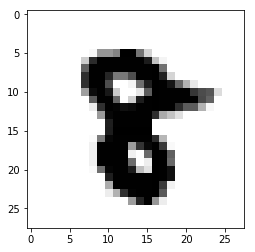
\includegraphics[width=\textwidth]{Images/input.png}
         \caption{Input image from the dataset.}
         \label{fig:nice_input}
     \end{subfigure} 
     \hfill
     \begin{subfigure}[b]{0.45\textwidth}
         \centering
         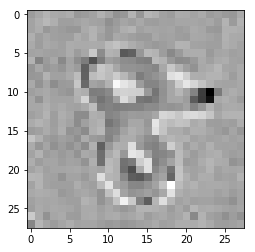
\includegraphics[width=\textwidth]{Images/transformed.png}
         \caption{Transformed after NF layers.}
         \label{fig:nice_transformed}
     \end{subfigure}
        \caption{NICE forward pass.}
        \label{fig:nice_forward}
\end{figure}

Given that the layers in a NF models are easily and cheaply invertible, it is trivial to obtain the original input image by performing a `\textit{backward}' pass through the model. 

Once the model is trained, it is then possible to generate new images by sampling from the known prior distribution $P_H$, and performing a backward pass through the model using the sampled vector. Figure \ref{fig:nice_sample} shows an example of a vector sampled from a Gaussian distribution ($P_H$) and the image generated by the model is shown in \ref{fig:nice_generated}.

\begin{figure}[htbp!]
     \centering
     \begin{subfigure}[b]{0.45\textwidth}
         \centering
         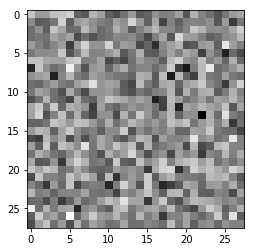
\includegraphics[width=\textwidth]{Images/sample.png}
         \caption{Vector sampled from $P_H$.}
         \label{fig:nice_sample}
     \end{subfigure} 
     \hfill
     \begin{subfigure}[b]{0.45\textwidth}
         \centering
         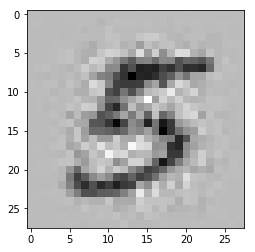
\includegraphics[width=\textwidth]{Images/generated.png}
         \caption{Generated from sampled vector.}
         \label{fig:nice_generated}
     \end{subfigure}
        \caption{NICE backward pass.}
        \label{fig:nice_backward}
\end{figure}

We trained our NICE implementation on the MNIST and FashionMNIST datasets. Figure \ref{fig:nice_results} shows some results from our experiments. The sampled vectors from the prior are show in the first column (Figure \ref{fig:nice_results_sampled2}). The middle (\ref{fig:nice_results_mnist2} and right columns (\ref{fig:nice_results_fashion2}) show the generated images when trained on MNIST and FashionMNIST, respectively. As can be appreciated, the same sampled vector will generate images belonging to different distributions depending on which dataset was used for training.

\begin{figure}[htbp!]
     \centering
     \begin{subfigure}[b]{0.3\textwidth}
         \centering
         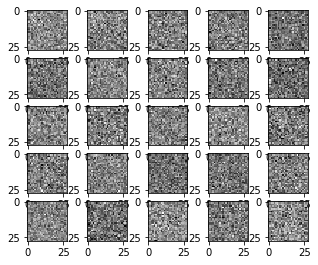
\includegraphics[width=\textwidth]{Images/prior1.png}
         %\caption{Sampled vectors}
         \label{fig:nice_results_sampled}
     \end{subfigure} 
     \hfill
     \begin{subfigure}[b]{0.3\textwidth}
         \centering
         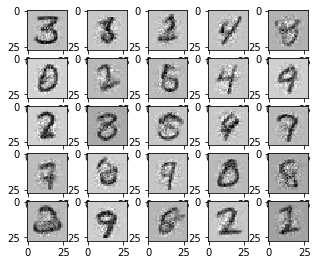
\includegraphics[width=\textwidth]{Images/mnist1.png}
         %\caption{MNIST}
         \label{fig:nice_results_mnist}
     \end{subfigure}
     \hfill
     \begin{subfigure}[b]{0.3\textwidth}
         \centering
         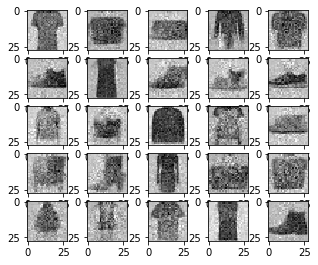
\includegraphics[width=\textwidth]{Images/fashion1.png}
         %\caption{FashionMNIST}
         \label{fig:nice_results_fashion}
     \end{subfigure}
     \\
     \begin{subfigure}[b]{0.3\textwidth}
         \centering
         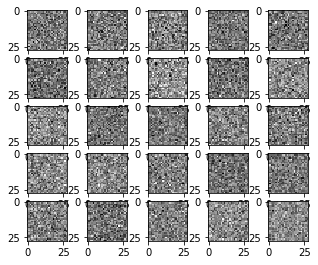
\includegraphics[width=\textwidth]{Images/prior2.png}
         \caption{Sampled vectors}
         \label{fig:nice_results_sampled2}
     \end{subfigure} 
     \hfill
     \begin{subfigure}[b]{0.3\textwidth}
         \centering
         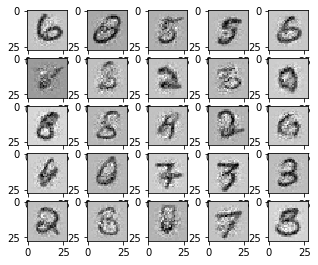
\includegraphics[width=\textwidth]{Images/mnist2.png}
         \caption{MNIST}
         \label{fig:nice_results_mnist2}
     \end{subfigure}
     \hfill
     \begin{subfigure}[b]{0.3\textwidth}
         \centering
         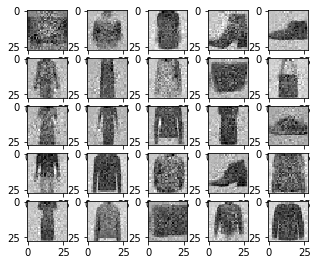
\includegraphics[width=\textwidth]{Images/fashion2.png}
         \caption{FashionMNIST}
         \label{fig:nice_results_fashion2}
     \end{subfigure}
        \caption{NICE results}
        \label{fig:nice_results}
\end{figure}
